%Have commented out sections that will be used but are not filled yet with %%%

\documentclass[10pt,letterpaper]{article}
\usepackage[latin1]{inputenc}
\usepackage{amsmath}
\usepackage{amsfonts}
\usepackage{amssymb}
%\usepackage{amsmacros}
\usepackage{graphicx}
%\usepackage{cite}
%\usepackage{siunitx}
\usepackage{placeins}% adds \FloatBarrier
%\providecommand{\e}[1]{\ensuremath{\times 10^{#1}}}% adds \e{}
%\usepackage{xcolor}
%\usepackage{pagecolor,lipsum}
%\usepackage{todonotes}% adds \listoftodos, \todo[]{}, and \missingfigure{}
%\usepackage{array}
%\usepackage{enumitem}

\newcommand{\td}{\todo[inline]}
\newcommand{\minus}[1]{\phantom{-} #1}

\renewcommand\thesection{\arabic{section}.}
\renewcommand\thesubsection{\hspace{0 em}(\alph{subsection})} % changed 2 em to 0 em
\renewcommand\thesubsubsection{\thesubsection\Roman{subsubsection}}

\newcommand{\lb}{[}
\newcommand{\rb}{]}
\newcommand{\comment}[2]{\hspace{0in}#2}

%\allowdisplaybreaks

%allows augmented matrix
\makeatletter
\renewcommand*\env@matrix[1][*\c@MaxMatrixCols c]{%
  \hskip -\arraycolsep
  \let\@ifnextchar\new@ifnextchar
  \array{#1}}
\makeatother

\usepackage{matlab-prettifier}


\begin{document}
\title{Lab 10}
\date{December 3, 2015}
\author{Boyd Esleck}
%\maketitle

\begin{eqnarray*}
f(x) &=& \sin\left(x^2 + \frac{x}{3}\right) \\
f'(x) &=& \left(2x + \frac{1}{3}\right)\cos\left(x^2 + \frac{x}{3}\right)  \\
\end{eqnarray*}


\begin{figure}
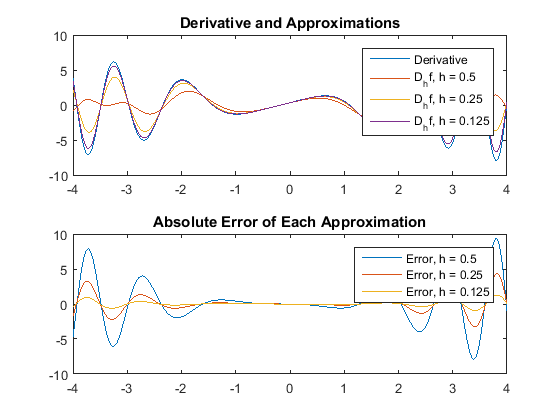
\includegraphics[width=\textwidth]{untitled}
\end{figure}
\FloatBarrier

\lstinputlisting[style = matlab-editor]{deriv_esleckbl.m}
\vspace{.25 in}
\hrulefill
\vspace{.25 in}
\lstinputlisting[style = matlab-editor]{func_esleckbl.m}

\end{document}